\usepackage{graphicx}
\usepackage{color}

\begin{document}

\pagenumbering{globe}

\begin{titlepage}

	\centering
	
\includegraphics{logo.png}

	\vspace{2\baselineskip}

	\LARGE{\textmd{ft\_hangouts}}
	\normalsize

	\LARGE{\textmd{The Great Ambassador}}
	\normalsize

	\vspace{2\baselineskip}

	Pierre-Elie Kesslassy pkesslas@student.42.fr

	\vspace{6\baselineskip}

	\textit{Summary: The goal of this project is to make you familiar with\
	Android system by creation a contact management application.}

	\pagestyle{empty}

\end{titlepage}

\tableofcontents

\pagestyle{empty}

\pagenumbering{arabic}

\raggedright

\section{Introduction}

In this project, you will need to make an Android application that will manage contacts and allow you to chat with them via SMS\@.

The goal of this project is to understand how an Android application works, how Android manages your application and how to use the SDK\@.

\centering

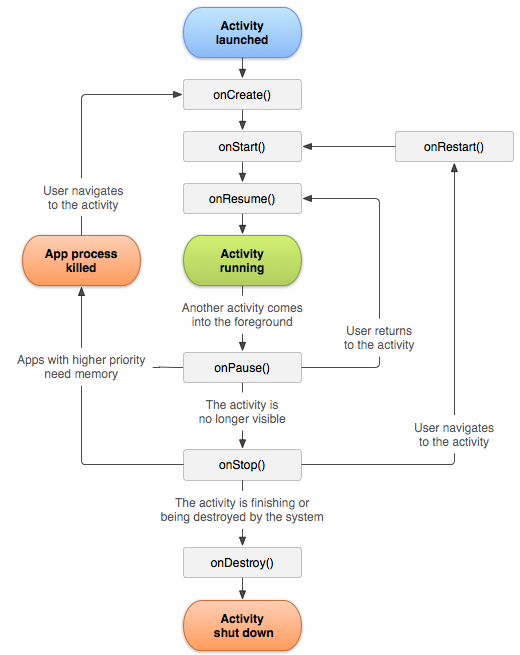
\includegraphics[height=10cm]{activity-lifecycle.png}

\raggedright

\section{Objectives}

You will have to perform various tasks that will make you understand how an Android application in JAVA or Kotlin. The goal is to make an application that allows to create a contact (with at least 5 information field), to edit it and to delete it. Once registered contact it will be possible to start dialogue with him via SMS\@.

Contacts must be persistently saved (in SQLite database, do not use the shared contact table, but create your own). A summary of each contact must be present on the application home list, a click on a summary must show all the information about the corresponding contact.

Your application will also have to work in two languages, one of which is default (change the language of the system to test). When you are on the home page and you set the application in the background, the date must be saved and displayed in a toast when you return app to the foreground. You must be able to change the color of the header of the application from preferences menu. And finally, the icon of the application must be the logo of 42.

\section{General Instructions}

\begin{itemize}
\tightlist{}
\item
  This project will only be corrected by humans.
\item
  The project should be in JAVA or Kotlin
\item
  No external library (even for design) is allowed.
\end{itemize}

\colorbox{red}{

	It is strongly recommended to use Android Studio as IDE. Be careful, the ADT plugin for Eclipse is no longer supported by Google.
}

\section{Mandatory Part}

Here's what you will need to do:

\begin{itemize}
\tightlist{}
\item
	Creation of the contact.
\item
	Edition of the contact.
\item
	Deletion of the contact.
\item
	Homepage with a summary of each contact.
\item
	Receiving SMS from saved contacts.
\item
	Sending SMS to your contacts.
\item
	Changing header color from menu.
\item
	Support of two languages.
\item
	Display the time of setting app to the background when you return to the application.
\item
	Landscape and portrait mode support.
\item
	The logo of the application must be 42.
\end{itemize}

\section{Bonus Part}

\begin{quote}
Bonuses will only be counted if your mandatory part is PERFECT. By
PERFECT, we obviously mean that it is fully realized, and it is not
possible to alter its behavior in default, even in case of error,
misuse, etc \ldots{} Concretely, this means that if your mandatory part
is not validated, your bonuses will be fully IGNORED.
\end{quote}

\begin{itemize}
\item
	Photo for contacts.
\item
	On sending an SMS to the new number, a contact with the number in name is directly created.
\item
	It's beautiful! Material Design is cool. (Without external libs such as ``AppCompat'' etc...).
\item
	Abillity to make call to the contact.
\end{itemize}

Be creative, lots of things can improve the application.

\section{Emulation}

This part explains how to use an Android emulator.

\begin{quote}
The emulator provided with Android Studio does not work for the moment. I recommended you to use Android Studio on a VM or a real device if you want to test SMS
\end{quote}

Several Android emulators exist, some more or less good: GenyMotion is very powerful and easy to set up (VirtualBox is required) but does not allow sending SMS in its free version.The AVD (Android Virtual Device) that comes with Android Studio is not the most powerful, but it gives more control. It is set up with Android Studio, and it's intuitive.

To send an SMS from the AVD\@:
\begin{verbatim}
gopa@e1r1p1$ telnet localhost {port, (window title)}
#Trying 127.0.0.1...
#Connected to localhost.
#Escape character is '^]'.
#Android Console: type 'help' for a list of commands
#OK
sms send {numero} {message}
\end{verbatim}

For a call:
\begin{verbatim}
gopa@e1r1p1$ telnet localhost {port, (window title)}
#[...]
gsm call {nubmer}
\end{verbatim}

When an image is running, the computer recognizes it as a phone. Choose that image when you launch the application from Android Studio.

\section{Correction and peer-evaluation}

Make your work on your GiT repository as usual. Only the present work on
your repository will be assessed in defense.

Beware of your repository, many more or less useful files are generated in your project. Remember to set up your .gitignore \href{https://www.gitignore.io/}{hint}.

For the correction the project will be compiled and installed with:
\begin{verbatim}
$./gradlew installDebug
\end{verbatim}
\end{document}
